\newpage
\begin{flushright}
    \textbf{\Large{Ujian Tengah Semester}}
    \subsection*{Tahun 2022}
    \addcontentsline{toc}{subsection}{UTS - 2022}
\end{flushright}
\vspace{0.5cm}
\hrule height 2pt
\vspace{0.5cm}
\begin{center}
    \textbf{\large{MATERI}}
    \begin{enumerate}[leftmargin=*, label={\arabic*}.]
        \item Menyelesaikan masalah turunan implisit.
        \item Menyelesaikan masalah turunan yang berkaitan.
        \item Mensketsa grafik fungsi dengan kalkulus.
    \end{enumerate}
\end{center}
\vspace{0.2cm}
\hrule height 1pt
\vspace{0.5cm}
\begin{center}
    \textbf{\large{SOAL}}
\end{center}
\begin{enumerate}[leftmargin=*, label={\arabic*}.]
\item 
\begin{enumerate}[label={\alph*}.]
    \item Dua sisi paralel dari suatu persegi panjang diperpanjang dengan laju 
    $2$ cm/dt. Sementara dua sisi lainnya diperpendek, sedemikian rupa sehingga 
    bentuknya tetap merupakan persegi dengan luas konstan $A=50$ cm$^2$.
    \begin{enumerate}[label={\roman*}.]
        \item Berapa laju keliling $P$ ketika panjang salah satu sisinya sekarang 
        adalah $10$ cm?
        \item Berapa panjang sisi-sisinya sekarang ketika keliling $P$ berhenti 
        berkurang?
    \end{enumerate}
    \item Misalkan diberikan $\ds\sin^{3}(x^2+y^2)+\frac{7x+\sin y^{2}}{x-1}=5$.
    Tentukan $\ds\frac{dy}{dx}$.
\end{enumerate}
\item Diketahui $f$ adalah fungsi berikut: $f(x)=x^{4}-4x^{3}+10$. Tentukan:
\begin{enumerate}[label={\alph*}.]
    \item Interval dimana fungsi $f$ naik dan turun.
    \item Nilai-nilai maksimum dan minimum lokal fungsi $f$ (jika ada).
    \item Interval dimana fungsi $f$ cekung ke atas dan cekung ke bawah.
    \item Titik-titik belok fungsi $f$ (jika ada).
    \item Sketsa Grafik fungsi $f$.
\end{enumerate}

\end{enumerate}
\vspace{0.2cm}
\hrule height 1pt
\vspace{0.5cm}
\begin{center}
    \textbf{\large{PEMBAHASAN}}
\end{center}
\begin{enumerate}[leftmargin=*, label={\arabic*}.]
\item
\begin{enumerate}[label={\alph*}.]
    \item Diberikan laju perpanjangan dua sisi paralel persegi panjang $2$ cm/dt dengan 
    luas konstan $50$ cm$^{2}$.

    Misalkan $x$ dan $y$ adalah panjang dan lebar persegi panjang, maka diperoleh persamaan
    \[
    A = xy \iff 50 = xy \iff y = \frac{50}{x}
    \]
    Diketahui pula rumus keliling adalah
    \[
    K = 2(x+y) = 2\bracket*{x+\frac{50}{x}}
    \]
    \begin{enumerate}[label={\roman*}.]
        \item Akan dicari laju keliling ketika panjang salah satu sisinya adalah $10$ cm.
        
        Dengan rumus keliling maka dengan mendiferensialkan kedua ruas diperoleh
        \begin{align*}
            \frac{dK}{dt} &= \drv{t}{2\bracket*{x+\frac{50}{x}}}\\
            &=2\bracket*{\frac{dx}{dt}+(-1)\frac{50}{x^{2}}\frac{dx}{dt}}\\
        \end{align*}
        Subtitusi laju perpanjangan $\ds \frac{dx}{dt} = 2$ dan panjang $x=10$.
        \begin{align*}
            \frac{dK}{dt} &=2\bracket*{(2)+(-1)\frac{50}{(10)^{2}}(2)}\\
            &=2\bracket*{2-\frac{100}{100}} = 2
        \end{align*}

        $\therefore$ Laju keliling ketika panjang salah satu sisinya adalah $10$ cm adalah
        $2$ cm/dt.
\begin{center}
    \line(1,0){150}
\end{center}

        
        \item Akan dicari panjang sisi-sisi $P$ ketika kelilingnya berhenti berkurang. 
        Sebelummnya diperoleh rumus keliling $K = 2(x+50/x)$. Keliling berhenti berkurang 
        ketika mencapai titik minimum. Sehingga akan dicari titik kritis dari $K$. Titik kritis 
        $K$ hanya terjadi pada titik stasioner. Sehingga
        \begin{align*}
            &\frac{dK}{dt} =2\bracket*{\frac{dx}{dt}+(-1)\frac{50}{x^{2}}\frac{dx}{dt}}\\
            \iff &0 = 2\bracket*{2-\frac{100}{x^{2}}}\\
            \iff &0 = 2x^{2}-100\\
            \iff &x^{2} = 50
        \end{align*}
        Maka diperoleh titik kritis $x=-\sqrt{50}$ dan $x=\sqrt{50}$. $x=-\sqrt{50}$ dapat 
        diabaikan karena nilai sisi $x$ harus positif. Sehingga tinggal membuktikan 
        $x=\sqrt{50}$ adalah titik minimum. Gunakan uji turunan kedua
        \begin{align*}
            \frac{d^{2}K}{dt^{2}} &= \drv{t}{2\bracket*{2-\frac{100}{x^{2}}}}\\
            &=0-(-2)\frac{200}{x^{3}} = \frac{400}{x^{3}}\\
            \Longrightarrow \frac{d^{2}K}{dt^{2}}\bracket*{\sqrt{50}} 
            &=\frac{400}{\bracket*{\sqrt{50}}^{3}} > 0
        \end{align*}
        Karena $\ds \frac{d^{2}K}{dt^{2}}\bracket*{\sqrt{50}} > 0$, maka dengan uji turunan kedua 
        $x=\sqrt{50} = 5\sqrt{2}$ adalah titik minimum.

        Diperoleh nilai $x$ sehingga keliling berhenti berkurang adalah $x=5\sqrt{2}$, lalu sisi 
        yang lainnya bernilai $y = 50/x = 5\sqrt{2}$.

        $\therefore$ Panjanga sisi-sisi $P$ ketika kelilingnya berhenti berkurang adalah 
        $5\sqrt{2}$ dan $5\sqrt{2}$. 
    \end{enumerate}
\begin{center}
    \line(1,0){150}
\end{center}
    \item Akan dicari $\ds\frac{dy}{dx}$ dari $\ds\sin^{3}(x^2+y^2)+\frac{7x+\sin y^{2}}{x-1}=5$.
    
    Turunkan secara implisit 
    \begin{align*}
        &\drv{x}{\sin^{3}(x^2+y^2)+\frac{7x+\sin y^{2}}{x-1}}=\drv{x}{5}\\
        \iff &\drv{x}{\sin^{3}(x^2+y^2)}+\drv{x}{\frac{7x+\sin y^{2}}{x-1}} = 0
    \end{align*}
    Selesaikan masing-masing turunan
    \begin{enumerate}[label={\arabic*})]
        \item \begin{align*}
        &\drv{x}{\sin^{3}(x^2+y^2)}\\
        =\,&3\sin^{2}(x^{2}+y^{2})\drv{x}{\sin(x^{2}+y^{2})}
        &\text{aturan rantai}\\
        =\,&3\sin^{2}(x^{2}+y^{2})\cos(x^{2}+y^{2})\drv{x}{x^{2}+y^{2}}
        &\text{aturan rantai}\\
        =\,&3\sin^{2}(x^{2}+y^{2})\cos(x^{2}+y^{2})\bracket*{2x+2y\frac{dy}{dx}}\\
        =\,&3\sin^{2}(x^{2}+y^{2})\cos(x^{2}+y^{2})(2x+2yy')
        \end{align*}
        \item \begin{align*}
            &\drv{x}{\frac{7x+\sin y^{2}}{x-1}} \\
            =\,&\frac{\drv{x}{7x+\sin y^{2}}(x-1)-(7x+\sin y^{2}\drv{x}{x-1})}{(x-1)^{2}}
            &\text{aturan pembagian}\\
            =\,& \frac{7+\cos y^{2}\drv{x}{y^{2}}}{x-1}-\frac{(7x+\sin y^{2})(1)}{(x-1)^{2}}
            &\text{turunkan dan aturan rantai}\\
            =\,&\frac{7+\cos y^{2}(2yy')}{x-1}-\frac{7x+\sin y^{2}}{(x-1)^{2}}
        \end{align*}
    \end{enumerate}
    Sehingga diperoleh 
    \begin{align*}
        &\drv{x}{\sin^{3}(x^2+y^2)}+\drv{x}{\frac{7x+\sin y^{2}}{x-1}} = 0\\
        \iff &3\sin^{2}(x^{2}+y^{2})\cos(x^{2}+y^{2})(2x+2yy') + 
        \frac{7+\cos y^{2}(2yy')}{x-1}-\frac{7x+\sin y^{2}}{(x-1)^{2}} = 0
    \end{align*}
    Misalkan 
    \begin{itemize}
        \item $A = 3\sin^{2}(x^{2}+y^{2})\cos(x^{2}+y^{2})$
        \item $B = 2y\cos y^{2}$
        \item $C = x-1$
        \item $D = 7x+\sin y^{2}$
    \end{itemize}
    Maka
    \begin{align*}
        &3\sin^{2}(x^{2}+y^{2})\cos(x^{2}+y^{2})(2x+2yy') + 
        \frac{7+\cos y^{2}(2yy')}{x-1}-\frac{7x+\sin y^{2}}{(x-1)^{2}} = 0\\
        \iff &A(2x+2yy')+\frac{By'+7}{C}-\frac{D}{C^{2}}=0\\
        \iff &2Ax+2Ayy' + \frac{B}{C}y' + \frac{7}{C} = \frac{D}{C^{2}}\\
        \iff &\bracket*{2Ay+\frac{B}{C}}y' = \frac{D}{C^2}-\frac{7}{C}-2Ax\\
        \iff &(2ACy+B)y' = \frac{D}{C}-7-2ACx\\
        \iff &(2ACy+B)y' = \frac{D-7C-2AC^{2}x}{C}\\
        \iff &y' =  \frac{D-7C-2AC^{2}x}{C(2ACy+B)}\\
    \end{align*}
    Subtitusi balik dan sederhanakan
    \begin{align*}
        y' &=  \frac{D-7C-2AC^{2}x}{C(2ACy+B)}\\
        &= \frac{\bracket*{7x+\sin y^{2}}-7(x-1)-2
        \bracket*{3\sin^{2}(x^{2}+y^{2})\cos(x^{2}+y^{2})}(x-1)^{2}x}{
        (x-1)\bracket*{2\bracket*{3\sin^{2}(x^{2}+y^{2})\cos(x^{2}+y^{2})}
        (x-1)y+2y\cos y^{2}}}\\
        &= \frac{\sin y^{2}+7-6x(x^{2}-2x+1)
        \bracket*{\sin^{2}(x^{2}+y^{2})\cos(x^{2}+y^{2})}}{
        6y(x^{2}-2x+1)\bracket*{\sin^{2}(x^{2}+y^{2})\cos(x^{2}+y^{2})}
        +2y(x-1)\cos y^{2}}
    \end{align*}

    $\therefore$ Turunan pertama dari $\ds\sin^{3}(x^2+y^2)+\frac{7x+\sin y^{2}}{x-1}=5$
    adalah
    
    $\ds \frac{dy}{dx} = \frac{\sin y^{2}+7-6x(x^{2}-2x+1)
    \bracket*{\sin^{2}(x^{2}+y^{2})\cos(x^{2}+y^{2})}}{
    6y(x^{2}-2x+1)\bracket*{\sin^{2}(x^{2}+y^{2})\cos(x^{2}+y^{2})}
    +2y(x-1)\cos y^{2}}$
\end{enumerate}
\begin{center}
    \line(1,0){300}
\end{center}
\item Diberikan $f(x)=x^{4}-4x^{3}+10$
\begin{enumerate}[label={\alph*}.]
    \item Akan dicari interval dimana fungsi $f$ naik dan turun.
    
    Fungsi $f$ naik ketika $f'(x) > 0$ dan turun ketika $f'(x) < 0$.\\
    Karena $f(x)=x^{4}-4x^{3}+10$ maka
    \[
    f'(x) = \drv{x}{x^{4}-4x^{3}+10} = 4x^{3}-12x^{2}
    \]
    Carilah titik stasioner $f$.
    \begin{align*}
        f'(x)=0 &\iff 4x^{3}-12x^{2}=0\\
        &\iff 4x^{2}(x-3) = 0
    \end{align*}
    Maka titik stasioner $f$ adalah $x=0$ dan $x=3$.
    \begin{center}
        \begin{tikzpicture}
            \draw[stealth-stealth] (-5,0) node[below]{$-\infty$}--(5,0) node[below]{$\infty$};
            \draw (-2,1)--(-2,-.1) node[below=0.2em]{$0$};
            \draw (2,1)--(2,-.1) node[below=0.2em]{$3$};
            
            \node at (3.5,1) {naik};
            \node at (-4,1) {turun};
            \node at (0,1) {turun};
            \node at (3.5,.5) {$+$};
            \node at (-4,.5) {$-$};
            \node at (0,.5) {$-$};
            \node [draw, shape = circle, fill = white, minimum size = 0.1cm, inner sep=0pt] at (2,0){};
            \node [draw, shape = circle, fill = white, minimum size = 0.1cm, inner sep=0pt] at (-2,0){};
            \node [draw, shape = circle, fill = white, minimum size = 0.1cm, inner sep=0pt] at (-2,0.15){};
            \end{tikzpicture}
    \end{center}
    Sehingga $f$ naik saat $x > 3$ dan $f$ turun saat $x < 3, x\neq 0$.

    $\therefore$ Interval dimana $f$ naik adalah $\ointervalo{3, \infty}$ dan interval dimana 
    $f$ turun adalah $\ointervalo{-\infty,0}\cup\ointervalo{0,3}$.
\begin{center}
    \line(1,0){150}
\end{center}
    \item Akan dicari nilai-nilai maksimum dan minimum lokal fungsi $f$ (jika ada).\\
    Titik kritis terjadi pada
    \begin{enumerate}[label={\arabic*})]
        \item Ujung interval
        \item Titik stasioner (saat $f'(c)=0$)
        \item Titik singular (saat $f'(c)$ tidak ada)
    \end{enumerate}
    Fungsi $f$ terdefinisi di bilangan real sehingga tidak memiliki ujung interval, dan bentuknya 
    juga polinomial sehingga tidak memiliki titik singular. Maka titik kritis hanya terjadi pada 
    titik stasioner yang telah diperoleh yaitu $x=0$ dan $x=3$. Gunakan uji turunan kedua 
    untuk menentukan apakah titik tersebut ekstrim.
    \[
        f''(x) = \drv{x}{4x^{3}-12x^{2}} = 12x^{2}-24x
    \]
    Subtitusi $x = 0$ dan $x = 3$ diperoleh $f''(0) = 0$ (bukan titik ekstrim), dan 
    $f''(3) = 36 > 0$ (titik ekstrim minimum). Diperoleh titik minimum di $x=3$ dengan nilai 
    $f(3) = -17$.

    $\therefore$ Nilai minimum lokal fungsi $f$ adalah $f(3)=-17$.
\begin{center}
    \line(1,0){150}
\end{center}
    \item Akan dicari interval dimana fungsi $f$ cekung ke atas dan cekung ke bawah.\\
    Fungsi $f$ cekung ke atas ketika $f''(x) > 0$ dan cekung ke bawah ketika $f''(x)<0.$
    Carilah titik stasioner $f'$.
    \begin{align*}
        f''(x)=0 &\iff 12x^{2}-24x=0\\
        &\iff 12x(x-2) = 0
    \end{align*}
    Maka titik stasioner $f'$ adalah $x=0$ dan $x=2$.=
    \begin{center}
        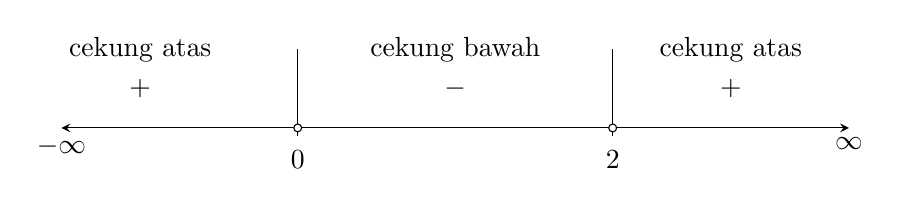
\begin{tikzpicture}
            \draw[stealth-stealth] (-5,0) node[below]{$-\infty$}--(5,0) node[below]{$\infty$};
            \draw (-2,1)--(-2,-.1) node[below=0.2em]{$0$};
            \draw (2,1)--(2,-.1) node[below=0.2em]{$2$};
            
            \node at (3.5,1) {cekung atas};
            \node at (-4,1) {cekung atas};
            \node at (0,1) {cekung bawah};
            \node at (3.5,.5) {$+$};
            \node at (-4,.5) {$+$};
            \node at (0,.5) {$-$};
            \node [draw, shape = circle, fill = white, minimum size = 0.1cm, inner sep=0pt] at (2,0){};
            \node [draw, shape = circle, fill = white, minimum size = 0.1cm, inner sep=0pt] at (-2,0){};
            \end{tikzpicture}
    \end{center}
    Sehingga $f$ cekung ke atas saat $x > 2 \cup x < 0$ dan $f$ cekung ke bawah saat 
    $0 < x < 2$.

    $\therefore$ Interval dimana $f$ cekung ke atas adalah$\ointervalo{-\infty,0}\cup\ointervalo{2,\infty}$ 
    dan interval dimana $f$ cekung ke bawah adalah $\ointervalo{0,2}$.
\begin{center}
    \line(1,0){150}
\end{center}
    \item Akan dicari titik belok fungsi $f$.\\
    Titik belok adalah titik pergantian dimana fungsi berubah dari cekung atas menjadi cekung bawah 
    atau sebaliknya. Dari ilustrasi pada jawaban sebelumnya terlihat bahwa titik belok terjadi saat 
    $x=0$ dan $x=2$.

    $\therefore$ Titk belok fungsi $f$ adalah $x=0$ dan $x=2$.
\begin{center}
    \line(1,0){150}
\end{center}
    \item Dengan hasil dari soal-soal sebelumnya, berikut hasil skesta fungsi $f$.
    \begin{center}
        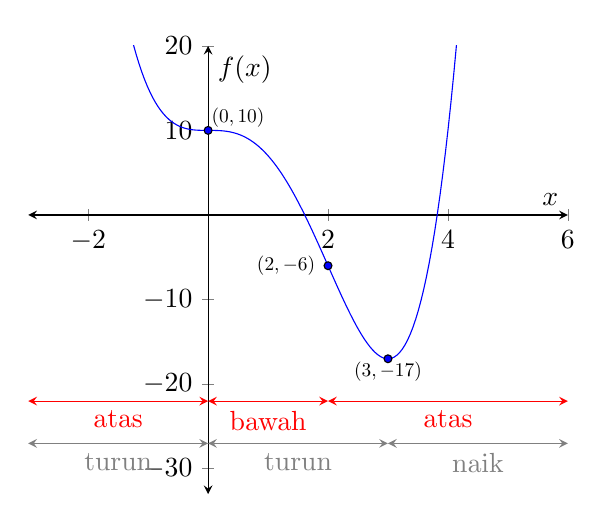
\begin{tikzpicture}[>=stealth]
        \begin{axis}[
            xmin=-3,xmax=6,
            ymin=-33,ymax=20,
            axis x line=middle,
            axis y line=middle,
            axis line style=<->,
            xlabel={$x$},
            ylabel={$f(x)$},
            ]
            \addplot[no marks,blue, -] expression[domain=-4:5,samples=200]{x^4-4*x^3+10};
            \node [draw, shape = circle, fill = blue, minimum size = 0.1cm, inner sep=0pt] at (3,-17){};
            \node at (3,-18.5){\scalebox{0.7}{$(3,-17)$}};
            \node [draw, shape = circle, fill = blue, minimum size = 0.1cm, inner sep=0pt] at (2,-6){};
            \node at (1.3,-6){\scalebox{0.7}{$(2,-6)$}};
            \node [draw, shape = circle, fill = blue, minimum size = 0.1cm, inner sep=0pt] at (0,10){};
            \node at (0.5,11.5){\scalebox{0.7}{$(0,10)$}};
            \draw[red, <->] (-3,-22) -- node[below](){atas} (0,-22);
            \draw[red, <->] (0,-22) -- node[below](){bawah} (2,-22);
            \draw[red, <->] (2,-22) -- node[below](){atas} (6,-22);
            \draw[gray, <->] (-3,-27) -- node[below](){turun} (0,-27);
            \draw[gray, <->] (0,-27) -- node[below](){turun} (3,-27);
            \draw[gray, <->] (3,-27) -- node[below](){naik} (6,-27);
        \end{axis}
        \end{tikzpicture}
        \end{center}

        $\therefore$ Telah disketsa fungsi $f$.
\end{enumerate}
\end{enumerate}

\begin{center}
    \line(1,0){300}
\end{center}